\section{Introduction}
\label{sec:intro}

\subsection{A short history of the effect}
\label{sec:history}
The equations governing a rotating rigid body with no torque acting on it were written down by Euler in the 1760s, and in 1834 Poinsot gave the geometric picture of the motion that is still used today: the angular momentum vector rolls along curves on the body's energy ellipsoid \cite{poinsot1834}.
From this analysis it follows that steady rotation about the axes of largest and smallest moment of inertia, the major and minor axes, is stable, while rotation about the intermediate axis is not.

The most famous observation came from space.
In June 1985 the cosmonauts Vladimir Dzha\-ni\-be\-kov and Viktor Savinykh flew Soyuz T-13 to the Salyut 7 space station, which had lost power and stopped responding to ground control months earlier.
They docked manually with the tumbling, frozen station and brought it back to life.
While unpacking supplies, Dzha\-ni\-be\-kov unscrewed a wing nut that spun off the end of its bolt and floated away.
As it drifted across the cabin, the nut flipped by \ang{180} every few seconds, again and again, while its spin stayed otherwise the same.
In microgravity there was nothing to cut the motion short, so the flips repeated periodically, which had never been seen so clearly before.
The phenomenon is now often called the \emph{Dzhanibekov effect} \cite{wiki_trt}.
Popular accounts claim the observation was kept quiet by the Soviet authorities for about a decade and was later linked to speculation that the Earth itself might flip over \cite{veritasium}.
We now know that the Earth won't flip over because it is already spinning about its major axis.

A related lesson had been learned earlier with Explorer 1, the first American satellite, launched in 1958.
It was designed to spin about its long axis, its \emph{minor} axis, but its flexible antennas dissipated energy and within hours it had moved to a tumble about its major axis.
For a body that is not perfectly rigid, only the major axis is truly stable.

The effect is easy to see on Earth.
A tennis racket, a book or a phone tossed in the air while spinning about its intermediate axis comes back having turned over by half a turn about another axis, while spins about the other two axes stay clean.
\begin{figure}[H]
    \centering
    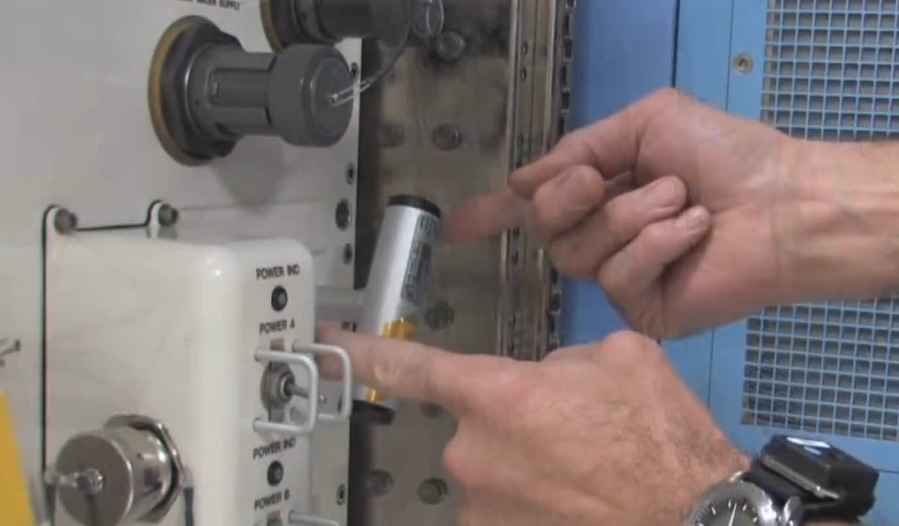
\includegraphics[width=0.6\linewidth]{Images/nasa_demo.jpeg}
    \caption{Demonstration of the effect by NASA astronauts in microgravity \cite{wiki_trt}.}
    \label{fig:intro}
\end{figure}

\makeatletter\if@firstcolumn\null\newpage\fi\makeatother\newpage % Theory starts on a new page (works from either column)
